\newcommand{\lpf}{
    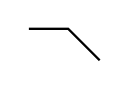
\begin{tikzpicture}[every path/.style={thick}]
        \draw (0,0) -- ++(0.5,0) -- ++(0.4, -0.4);
    \end{tikzpicture}
}

\newcommand{\quantizer}{
    \begin{tikzpicture}[every path/.style={thick}]
        \draw (0  ,  0) -- ++(0.2, 0) -- ++(0, 0.2);
        \draw (0.2,0.2) -- ++(0.2, 0) -- ++(0, 0.2);
        \draw (0.4,0.4) -- ++(0.2, 0) -- ++(0, 0.2);
        \draw (0.6,0.6) -- ++(0.2, 0);
    \end{tikzpicture}
}

\newcommand{\onebitq}{
    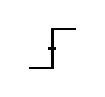
\begin{tikzpicture}[every path/.style={thick}]
        \draw (0  ,  0) -- ++(0.3, 0) -- ++(0, 0.5) -- ++(0.3, 0);
        \draw (0.25  ,  0.25) -- (0.35, 0.25);
    \end{tikzpicture}
}

\newcommand{\onebitqrev}{
    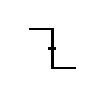
\begin{tikzpicture}[every path/.style={thick}]
        \draw (0.0  ,  0.5) -- ++(0.3, 0) -- ++(0, -0.5) -- ++(0.3, 0);
        \draw (0.25  ,  0.25) -- (0.35, 0.25);
    \end{tikzpicture}
}


\newcommand{\onebitqthick}{
    
\begin{tikzpicture}[every path/.style={ultra thick}]
        \draw (0  ,  0) -- ++(0.3, 0) -- ++(0, 0.5) -- ++(0.3, 0);
        \draw (0.2  ,  0.25) -- (0.4, 0.25);
    \end{tikzpicture}
}

% \newcommand{\veconebitq}{
%     \begin{tabular}{ c }
%         \begin{tikzpicture}[every path/.style={thick}]
%             \draw (0  ,  0) -- ++(0.2, 0) -- ++(0, 0.4) -- ++(0.2, 0);
%             \draw (0.15  ,  0.2) -- (0.25, 0.2);
%         \end{tikzpicture}  \\
%         \vdots \\
%         \begin{tikzpicture}[every path/.style={thick}]
%             \draw (0  ,  0) -- ++(0.2, 0) -- ++(0, 0.4) -- ++(0.2, 0);
%             \draw (0.15  ,  0.2) -- (0.25, 0.2);
%         \end{tikzpicture}
%     \end{tabular}

% }


\newcommand{\ci}{
\begin{tabular}{ c }
    $\int$  \\
    \vdots \\
    $\int$
\end{tabular}
}

\newcommand{\dec}{
\begin{tikzpicture}[transform shape, scale=0.35]
    \draw[thick] (0,0) .. controls (0.98,0) .. (1,-2) to[out=90,in=90] ++(4mm, 0) to[out=90,in=90] ++(4mm, 0) to[out=90,in=90] ++(4mm, 0);
    \draw[arrow, ultra thick] (1.8,0.2) -- (1.8,-1.1);
\end{tikzpicture}

}
